This section presents the final TRITIUM monitor, a schematic design of which is shown in Figure \ref{fig:TritiumDetectorSchematicDesign}. It consists of a number of TRITIUM modules read out in parallel, the design of each one will include the characteristics (differences between the latest prototypes) with which the best results has been obtained. These modules are shielded from environmental radioactivity by three different techniques:

\begin{enumerate}

\item{} An external lead shield, which is used to stop the environmental radioactivity and soft cosmic rays (particles with energies below $200~\MeV$).

\item{} Several active vetos, which are placed below and above the TRITIUM modules. These active vetos are read out in anticoincidence to supress high energy event background, mainly cosmic ray particles with energies above $200~\MeV$.

\item{} A water purification system, which is used to eliminate the radioactive elements present in the water samples measured by the TRITIUM monitor.

\end{enumerate}

\begin{figure}[h]
\centering
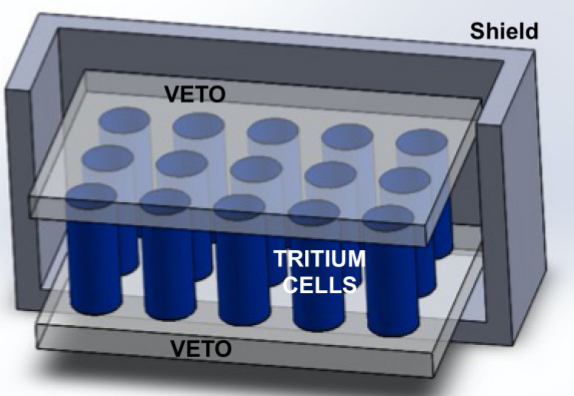
\includegraphics[scale=0.5]{5Prototypes/55ModularTritiumDetector/FinalTritium.png}
\caption{A schematic design of the TRITIUM detector.\label{fig:TritiumDetectorSchematicDesign}}
\end{figure}

The water purification system, the lead shield and a TRITIUM-Aveiro prototype are installed and currently in operation at the Arrocampo dam. This entire system is employed to successfully monitor the tritium levels in Arrocampo dam during several months. Furthermore, two additional TRITIUM-Aveiro prototypes and four active vetos are currently under construction and will be measured in parallel with this prototype.

The electronics of the TRITIUM-Aveiro prototype, based on a RaspberryPi, cannot be used for multiple modules due to counting limitations and this must be replaced by an FPGA-based counter board.

Three TRITIUM-IFIC-2 prototypes and two active veto (on up and other below the modules) are already built and they will be installed as soon as possible. In this first installation, lateral cosmic vetos for the TRITIUM-IFIC-2 modules are not contemplated since its influence is expected to be small ($\propto \text{cos}^2(\theta)$), but if necessary they can be included in the future.

One of the most important aspects of the TRITIUM monitor is its modular design, which allows scalability to reach the required sensitivity, $100~\becquerel/\liter$. It means that if this target sensitivity is not achieved with the three modules to be installed, it can be obtained by installing additional modules.

The only scalability restriction is the available space, which is set by the lead shield and the cabin in which the setup is installed. In the currently available space, five different structures as the one shown in Figure \ref{fig:TritiumMonitorIFIC2Design} can be placed, each one containing 10 modules and two active veto. If the 50 TRITIUM modules are installed, the sensitivity of the TRITIUM monitor could be improved by a factor of around 7 ($\sqrt{50}$) with respect to the sensitivity of a single module.

\begin{figure}[h]
\centering
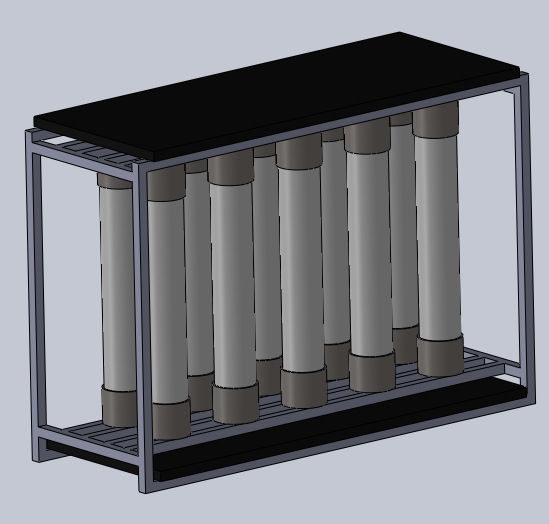
\includegraphics[scale=0.6]{5Prototypes/55ModularTritiumDetector/Tritium_Detector_Based_On_Tritium_IFIC_2.PNG}
\caption{A TRITIUM monitor design based on the TRITIUM-IFIC-2 prototype.\label{fig:TritiumMonitorIFIC2Design}}
\end{figure}